\documentclass[twoside,a4paper]{article}
\usepackage{geometry}
\geometry{margin=1.5cm, vmargin={0pt,1cm}}
\setlength{\topmargin}{-1cm}
\setlength{\paperheight}{29.7cm}
\setlength{\textheight}{25.3cm}

% useful packages.
\usepackage{amsfonts}
\usepackage{amsmath}
\usepackage{amssymb}
\usepackage{amsthm}
\usepackage{enumerate}
\usepackage{graphicx}
\usepackage{multicol}
\usepackage{fancyhdr}
\usepackage{layout}

% some common command
\newcommand{\dif}{\mathrm{d}}
\newcommand{\avg}[1]{\left\langle #1 \right\rangle}
\newcommand{\difFrac}[2]{\frac{\dif #1}{\dif #2}}
\newcommand{\pdfFrac}[2]{\frac{\partial #1}{\partial #2}}
\newcommand{\OFL}{\mathrm{OFL}}
\newcommand{\UFL}{\mathrm{UFL}}
\newcommand{\fl}{\mathrm{fl}}
\newcommand{\op}{\odot}
\newcommand{\Eabs}{E_{\mathrm{abs}}}
\newcommand{\Erel}{E_{\mathrm{rel}}}

\begin{document}

\pagestyle{fancy}
\fancyhead{}
\lhead{NAME Jiatu Yan}
\chead{Numerical Analysis homework \#3}
\rhead{Date 2020.4.5}


\section*{I. \small{Using Newton's formula on $f\left( x \right)=\frac{1}{1+x^2} $}}
\begin{figure}[h]
	\centering
	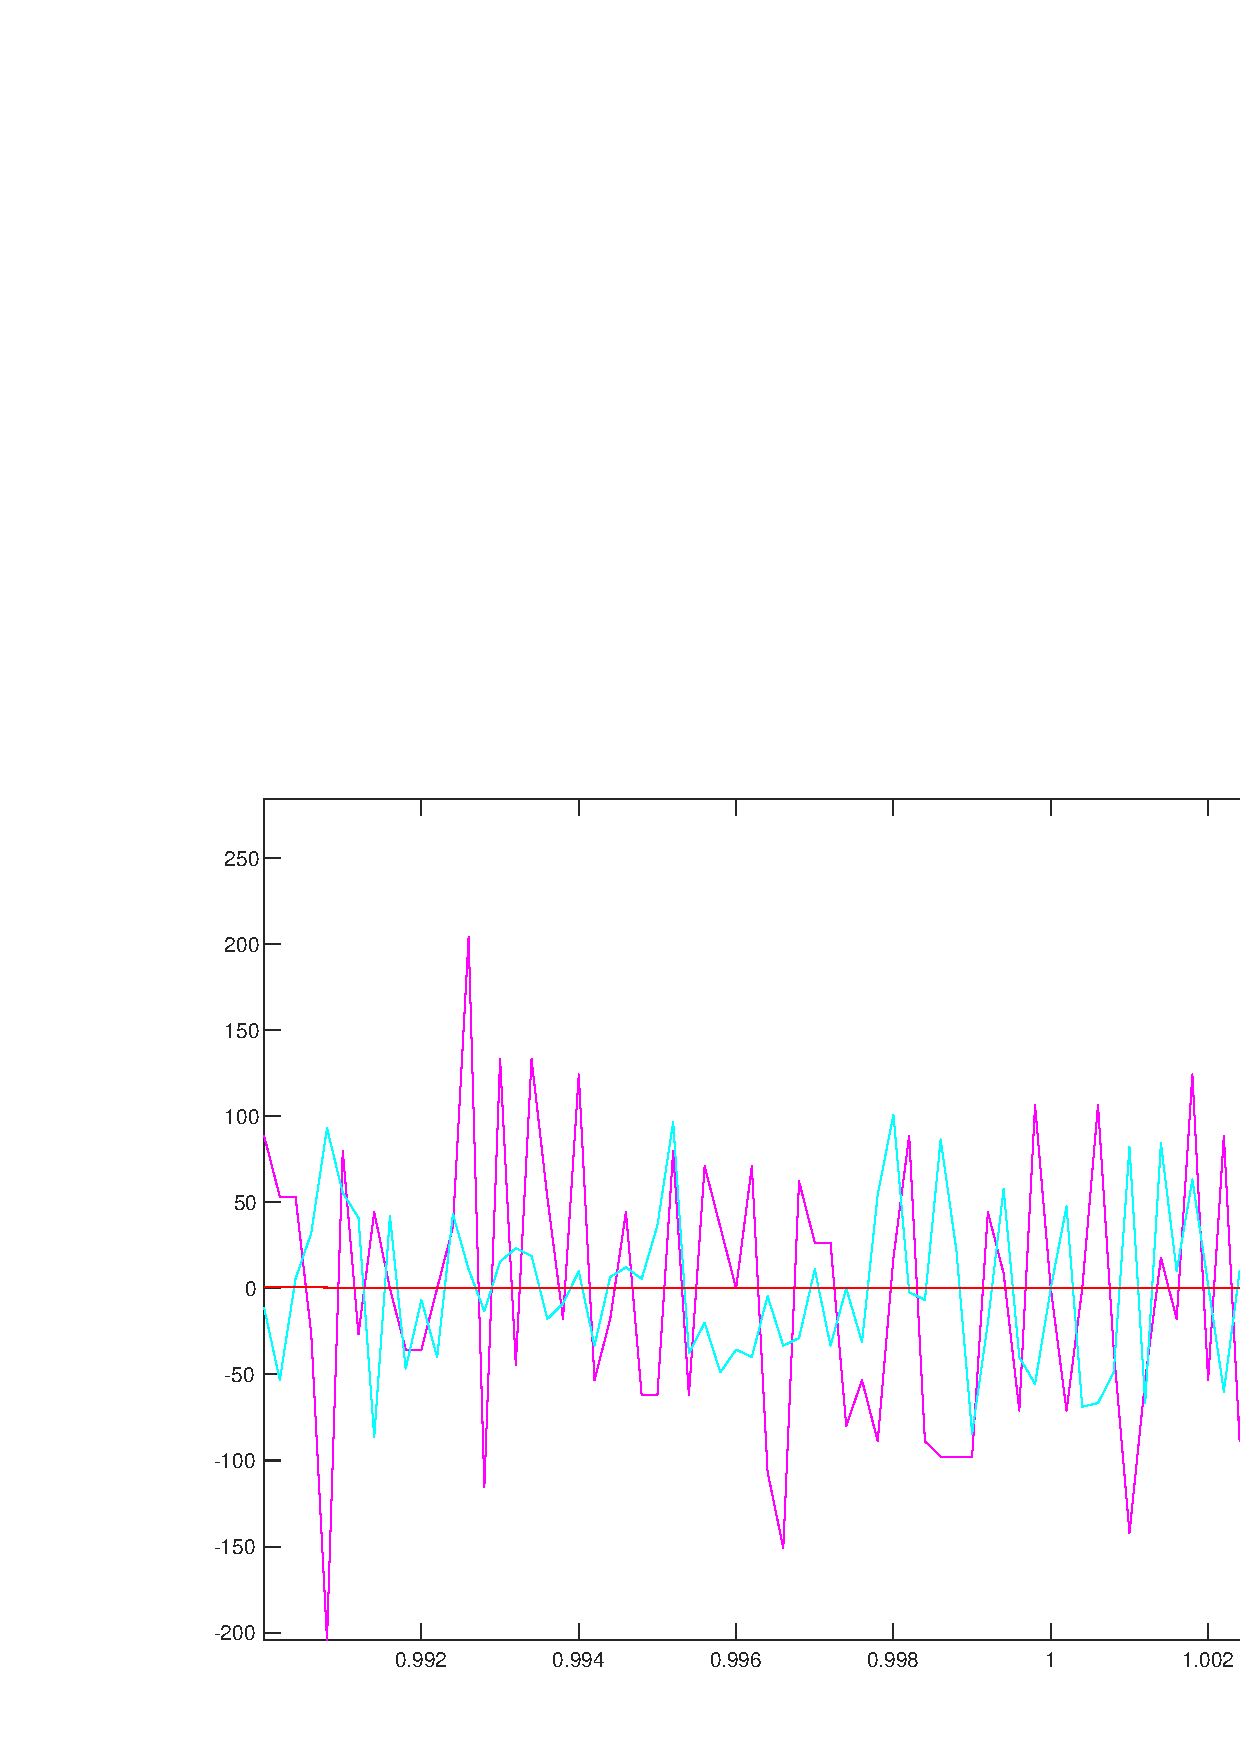
\includegraphics[width=10cm,height=5cm]{Plot1.png}
	\caption{The Runge phenomenon.}
\end{figure}
We can find that the polynomials are not uniformly convergent to $f(x)$.

\section*{II. \small{Perform Chebyshev interpolation for $f\left( x \right)=\frac{1}{1+25x^2} $}}

\begin{figure}[h]
        \centering
        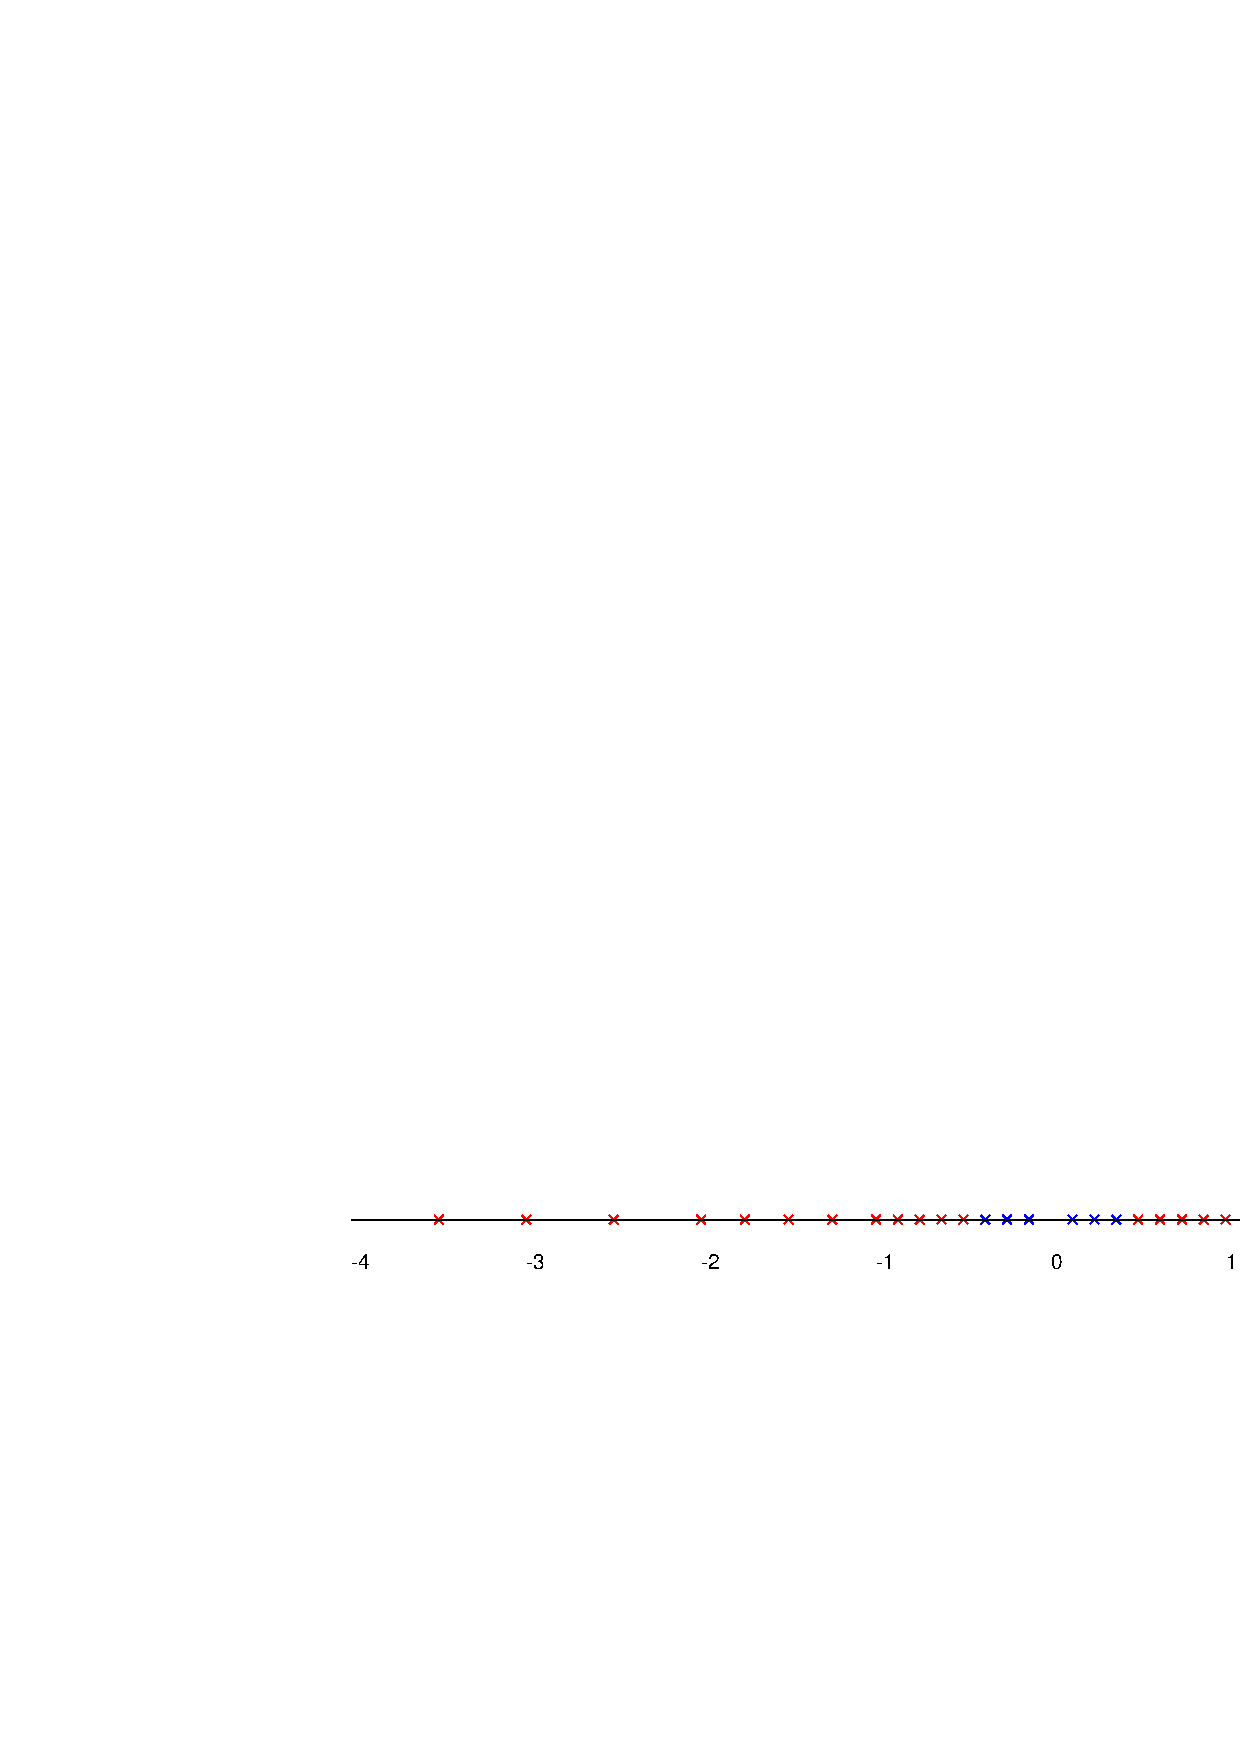
\includegraphics[width=10cm,height=5cm]{Plot2.png}
        \caption{Chebyshev interpolation.}
\end{figure}

By using Chebyshev interpolation, the polynomials uniformly converges to $f(x)$
, so it is free of the wide oscillations in section I.
\end{document}

%%% Local Variables: 
%%% mode: latex
%%% TeX-master: t
%%% End: 
